% interactcadsample.tex
% v1.03 - April 2017

\documentclass[]{interact}

\usepackage{epstopdf}% To incorporate .eps illustrations using PDFLaTeX, etc.
\usepackage{subfigure}% Support for small, `sub' figures and tables
%\usepackage[nolists,tablesfirst]{endfloat}% To `separate' figures and tables from text if required

\usepackage{natbib}% Citation support using natbib.sty
\bibpunct[, ]{(}{)}{;}{a}{}{,}% Citation support using natbib.sty
\renewcommand\bibfont{\fontsize{10}{12}\selectfont}% Bibliography support using natbib.sty

\theoremstyle{plain}% Theorem-like structures provided by amsthm.sty
\newtheorem{theorem}{Theorem}[section]
\newtheorem{lemma}[theorem]{Lemma}
\newtheorem{corollary}[theorem]{Corollary}
\newtheorem{proposition}[theorem]{Proposition}

\theoremstyle{definition}
\newtheorem{definition}[theorem]{Definition}
\newtheorem{example}[theorem]{Example}

\theoremstyle{remark}
\newtheorem{remark}{Remark}
\newtheorem{notation}{Notation}

% see https://stackoverflow.com/a/47122900

% Pandoc citation processing

\usepackage{hyperref}
\usepackage[utf8]{inputenc}
\def\tightlist{}


\begin{document}

\articletype{Preprint}

\title{Continuing COVID-19 Vaccination of Front-Line Workers in BC with
the AstraZeneca Vaccine: Benefits in the Face of Increased Risk for
Prothrombotic Thrombocytopenia}


\author{\name{Amin Adibi$^{a}$, Mohsen Sadatsafavi$^{a}$}
\affil{$^{a}$Respiratory Evaluation Sciences Program, Faculty of
Pharmaceutical Sciences, University of British Columbia, Vancouver, BC,
Canada}
}

\thanks{CONTACT Amin
Adibi. Email: \href{mailto:amin.adibi@ubc.ca}{\nolinkurl{amin.adibi@ubc.ca}}, Mohsen
Sadatsafavi. Email: \href{mailto:Mohsen.Sadatsafavi@ubc.ca}{\nolinkurl{Mohsen.Sadatsafavi@ubc.ca}}}

\maketitle

\begin{abstract}
Recently, the National Advisory Committee on Immunization (NACI)
recommended against using the AstraZeneca COVID-19 vaccine pending
further review of the risk for Vaccine-Induced Prothrombotic Immune
Thrombocytopenia (VIPIT). Using straightforward calculations and based
on current evidence, we propose that even if the risk is found to be
causally related to the AstraZeneca vaccine, the benefits of continuing
immunization of essential workers with AstraZeneca by far outweigh the
risk. We consider the case of British Columbia as an example. The
province is expected to received an addtional 246700 doses of
AstraZeneca vaccine through US and COVAX until April 11th, enough to
provide the first dose of vaccine to all unvacinated front-line workers.
We estimate that if British Columbia continues the front-line worker
vaccination program with the AstraZeneca vaccine, we expect to see 2
VIPIT-related deaths, 40,000 fewer cases of COVID-19, 500 fewer
hospitalizations, 100 fewer deaths, and 1,800 fewer cases of Long COVID
even if all essential workers were under 55 and assuming the highest
estimated rate of 1 in 100,000 currently reported for VIPIT.
\end{abstract}

\begin{keywords}
COVID19; astrazeneca; vaccination; essentialworkers; clots;
thrombocytopenia; harm-benefit; BC
\end{keywords}

\hypertarget{background}{%
\section{Background}\label{background}}

Recently, NACI recommended against using AstraZeneca COVID-19 Vaccine
for Canadians under the age of 55, due to concerns about the incidence
of Vaccine-Induced Prothrombotic Immune Thrombocytopenia (VIPIT) based
on European reports \citep{naci_naci_2021}. On Match 18, 2021, the
European Medicines Agency estimated the incidence of VIPIT at
approximately 1 per 1,000,000 people vaccinated with the AstraZeneca
vaccine \citep{ema_covid-19_2021}. A higher estimated rate of 1 per
100,000 by the Paul-Ehrlich Institut in Germany was published on March
19th \citep{pei_covid-19_2021}. It was this higher rate reported by the
Paul-Ehrlich Institut that led NACI to recommend against using this
vaccine in adults under 55 years old \citep{naci_naci_2021}. BC had
initially slated the AstraZeneca vaccine for outbreak control and
front-line workers vaccination program. on March 29th and following
NACI's recommendation, BC paused using the AstraZeneca vaccine for those
under 60 and put the front-line workers vaccination program on hold.

On April 1st, the UK Medicines \& Healthcare Products Regulatory Agency
updated its own previously reported data to report a total of 22
cerebral venous sinus thrombosis (CVST) and 8 other clot-related events
from 18.1 million doses of the AstraZeneca vaccine (total incidence rate
1 in 600,000) \citep{mhra_coronavirus_2021}.

Canadian provinces are expected to receive 1.5 million doses of the
AstraZeneca vaccine from the US and another 316,800 doses from the COVAX
program between now and April 11th
\citep{government_of_canada_vaccines_2021}. British Columbia expects to
receive 246,700 doses from these two AstraZeneca deliveries, enough to
finish providing the first dose to all remaining front-line workers.

The 300,690 doses of Pfizer-BioNTech and 105,900 doses of Moderna
vaccines expected within the same time frame are currently allocated for
the priority groups, indigenous population, and age-based vaccination
campaign currently vaccinating those in their 70s. The AstraZeneca
vaccine was initially slated for essential workers due to its easier
handling and storage requirements. If it is logistically possible to
switch the vaccine allocation for above 55 years old age groups to the
AstraZeneca vaccine and use either Pfizer-BioNTech or Moderna vaccines
for younger front-line workers without delay, that might be the
preferred approach. However, if that is not logistically feasible, one
might ask whether the benefits of deploying the AstraZeneca vaccine for
front-line workers outweigh the rate but serious risk for VIPIT.

Harm-benefit of the administering the AZ doses to younger front-line
workers can be analyzed from either a societal or a personal
perspective. From a societal perspective and assuming a utilitarian
framework, we can estimate compare outcomes such as deaths, life years
lost, or Quality-Adjusted Life Years (QALYs) under different scenarios.
However, a net-beneficial intervention at the societal level does not
necessary translate to a net-benefit at the personal level, as the those
who carry the burden of risk may be different from those who are likely
to benefit from the intervention.

Whether explicitly stated or not, the choice of the outcome is affected
by value judgments as well. Choosing life-years lost as an outcome, for
instance, favours younger people. To make things more complex, roll-out
decisions can get tangled in all sorts of societal issues, including
public trust in not only COVID-19 vaccines but vaccine hesitancy in
general.

Here, we provide a preliminary harm-benefit analysis of immediate
vaccination of all front-line workers with the AstraZeneca COVID-19
vaccine. We based our analysis on mortality alone, and explore the risk
both from a societal and personal perspective, and touch on some
important ethical and practical considerations.

\hypertarget{methods}{%
\section{Methods}\label{methods}}

We estimated benefits of the AstraZeneca COVID-19 matrix using a
BC-specific age-structured COVID-19 compartmental model by Mulberry and
colleagues that takes into account transmission, age-based contact
structure, front-line worker status, and rising \(R_0\) due to variants
of concern \citep{mulberry_vaccine_2021}. The model included
susceptible, exposed, infectious and recovered (SEIR) status and was
based on the transmission model by Bubar et al
\citep{bubar_model-informed_2021}.

We ran the model from January 2021 to September 2021, which is when
expect the vaccination campaign to conclude. To follow BC vaccination
strategy and case counts in the first three months of 2021, we held
\(R_0\) at 1.05 from January 1, 2021 for 90 days during which people
over 80 years old followed by those between 70-79 years old became
eligible for vaccination. Age groups that were offered vaccination were
considered to be vaccinated at a steady pace until everyone who is not
vaccine-hesitant is vaccinated. Around the end of March, we raised
\(R_0\) to either 1.15 or 1.3 to account for variants of concern gaining
a foothold in BC.

We assumed the first dose of the vaccine, regardless of the
manufacturer, to offer a 90\% efficacy against serious illness. We
further assume that all British Columbians will be offered a first dose
before July 1st, 2021, and a second dose before the end of September
2021. We assumed that each dose of the AstraZeneca vaccine to be
independently associated with the highest reported risk for VIPIT. We
did not consider the risk for anaphylaxis, as all vaccines seem to have
a similar risk in that regard and the risk can be mitigated in the
vaccination clinic.

For harm-benefit analysis from a societal perspective, we compared
expected number of deaths under each vaccination strategy. For
harm-benefit analysis from a personal perspective, we compared the
mortality risk due to VIPIT with mortality risk from COVID-19 due to
delayed vaccination in each age group. We assumed the risk from VIPIT to
be constant across all age groups under 60.

All the analysis was performed using publicly-available data and code.
This manuscript is produced by a reproducible R Markdown script, which
is available on
\href{https://github.com/aminadibi/astrazenecaVIPIT}{Github}.

\hypertarget{results}{%
\section{Results}\label{results}}

\begin{figure}

{\centering 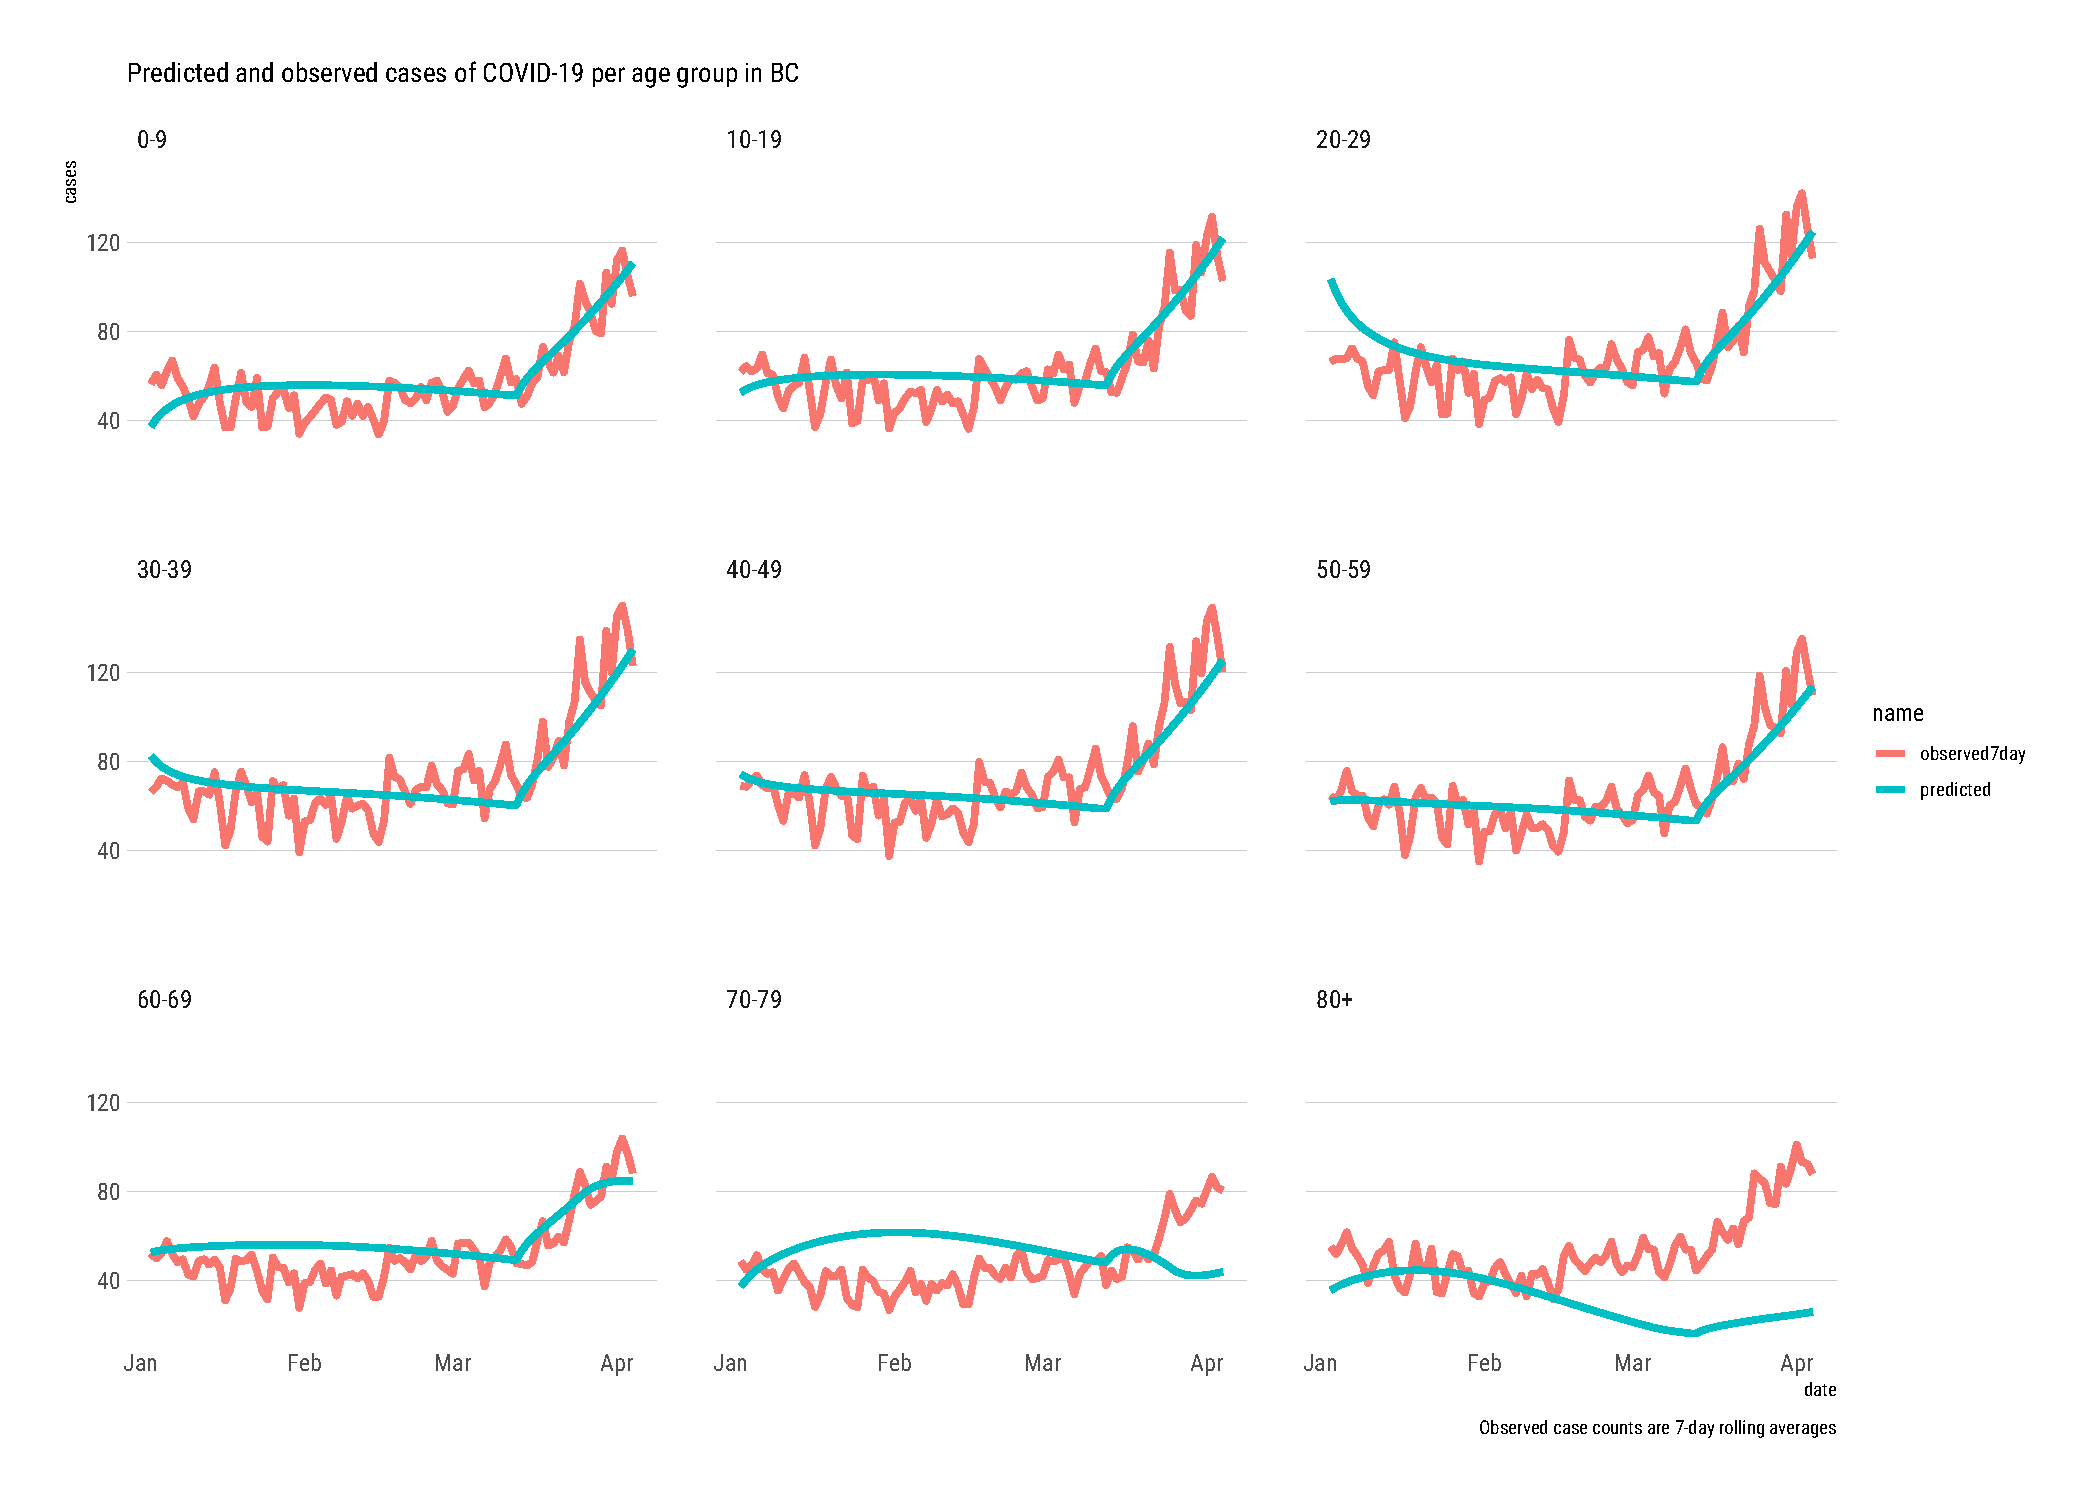
\includegraphics[width=1\linewidth]{../figures/fig-validation} 

}

\caption{Face validity of model case counts}\label{fig:figValidation}
\end{figure}

Predicted epidemiological curve and age-stratified case counts showed
good agreement with observed counts reported by BC CDC, as shown in
Figure 1.

\begin{table}
\tbl{Harm-benefit parameters and their distribution }
{\begin{tabular}{lccc} \toprule
 & \multicolumn{2}{l}{Estimates} \\ \cmidrule{2-4}
 Variable & Base Value & Probability Distribution & Source \\ \midrule
 Rate of VIPIT\textsuperscript{a} & 1 in 153,000 & $\beta(222, 3.4\times 10^7)$ & EudraVigilance  \\
 VIPIT Mortality Risk & $40\%$ & $\beta(4, 10)$ & NACI  \\
 Gamma & C2 & C2 & C3  \\ \bottomrule
\end{tabular}}
\tabnote{\textsuperscript{a}This footnote shows how to include
 footnotes to a table if required.}
\label{sample-table}
\end{table}

\hypertarget{harm-benefit-from-a-societal-perspective}{%
\subsection{Harm-Benefit From A Societal
Perspective}\label{harm-benefit-from-a-societal-perspective}}

Assuming that BC allocates all 246,700 doses to front-line workers, we
can estimate the expected number of deaths due to VIPIT,
\(E(death)_{VIPIT}\), as shown below. To err on the side of caution, we
assume that each dose of the vaccine is independently associated with
the risk for VIPIT and that all recipients are under 55 and as such at
higher risk for VIPIT. We also assume that there is enough uptake that
BC is able to administer all these doses.

\[
E(death)_{VIPIT}  = n \times d \times P(VIPIT|AZ) \times P(death|VIPIT, AZ)
\] where \(n\) is the number of vaccine recipients, \(d\) is the number
of doses administered per person, \(P(VIPIT|AZ)\) is the risk of VIPIT
after receiving each dose, and \(P(death|VIPIT, AZ)\) is the case
fatality for VIPIT.

To err on the side of caution, we will follow NACI's lead and assume the
highest reported rate of VIPIT, which is 1 in 100,000 recipients, so
\(P(VIPIT|AZ) = \frac{1}{100,000}\). On the other hand, as reported by
NACI, case fatality due to VIPIT is currently estimated at 40\% but is
likely to decrease as there will be more awareness and better early
treatment. Again to err on the side of caution, we'll keep the estimate
at 40\%: \(P(death|VIPIT, AZ)=40\%\)

\[
\begin{aligned}
E(death)_{VIPIT} & = n \times 2 \times \frac{1}{100,000} \times \frac{40}{100} \\
& = 246,700 \times \frac{8}{1,000,000} \\
& \approx 2  
\end{aligned}
\]

The expected number of mortality under the scenario of immediately
offering the AstraZeneca vaccine to all front-line workers is 2 persons
in BC.

\begin{figure}

{\centering 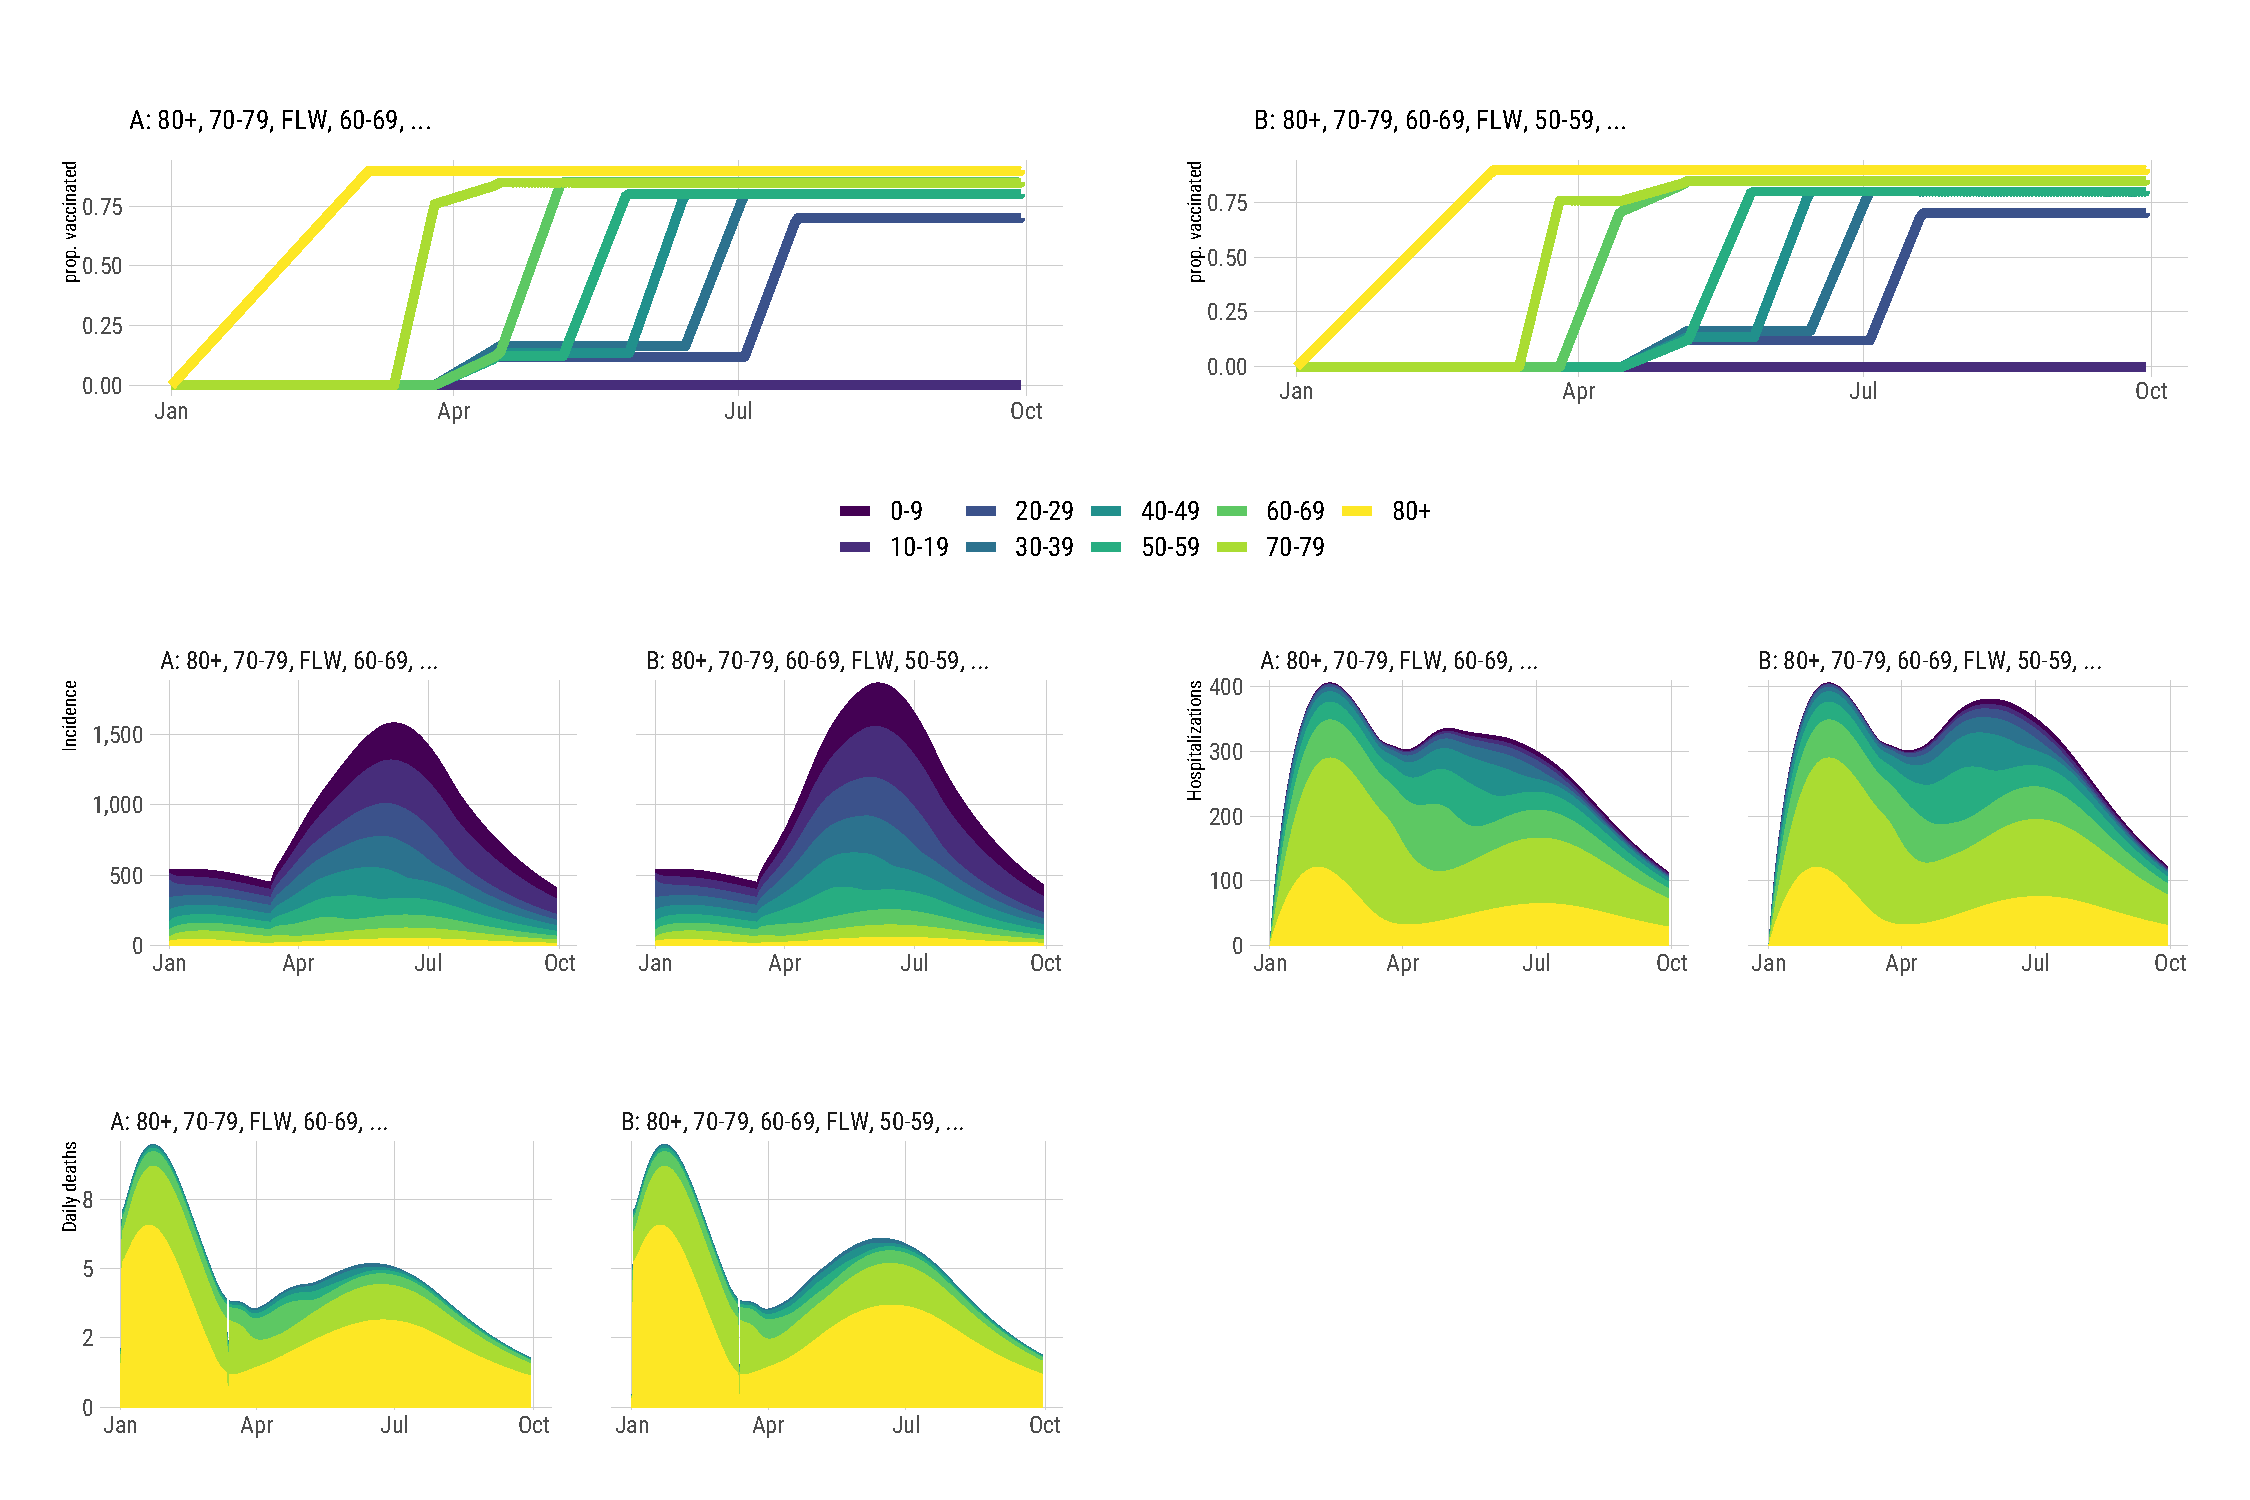
\includegraphics[width=1\linewidth]{../figures/fig-trajectoriesFull} 

}

\caption{Projection of the Progression of the Vaccination Program and COVID-19}\label{fig:fig1}
\end{figure}

We used a compartmental model of transmission and vaccination of
COVID-19 in BC to estimate benefits of immediately continuing the
front-line workers vaccination program using the AstraZeneca vaccine.

We compared immediately prioritizing essential workers for a vaccine
(Scenario A) and delaying it until after those over 70 are fully
vaccinated (Scenario B).

In our analysis, scenario A led to 38471 fewer cases of COVID-19, 754
fewer hospitalizations, 183 fewer deaths, and 2149 fewer cases of Long
COVID, assuming \(R_0=1.3\) and that vaccine effeteness in preventing
transmission is on average 60\%. Figure 3 shows results for a wider
range of \(R_0\) and efficacy against infection values.

\begin{figure}

{\centering 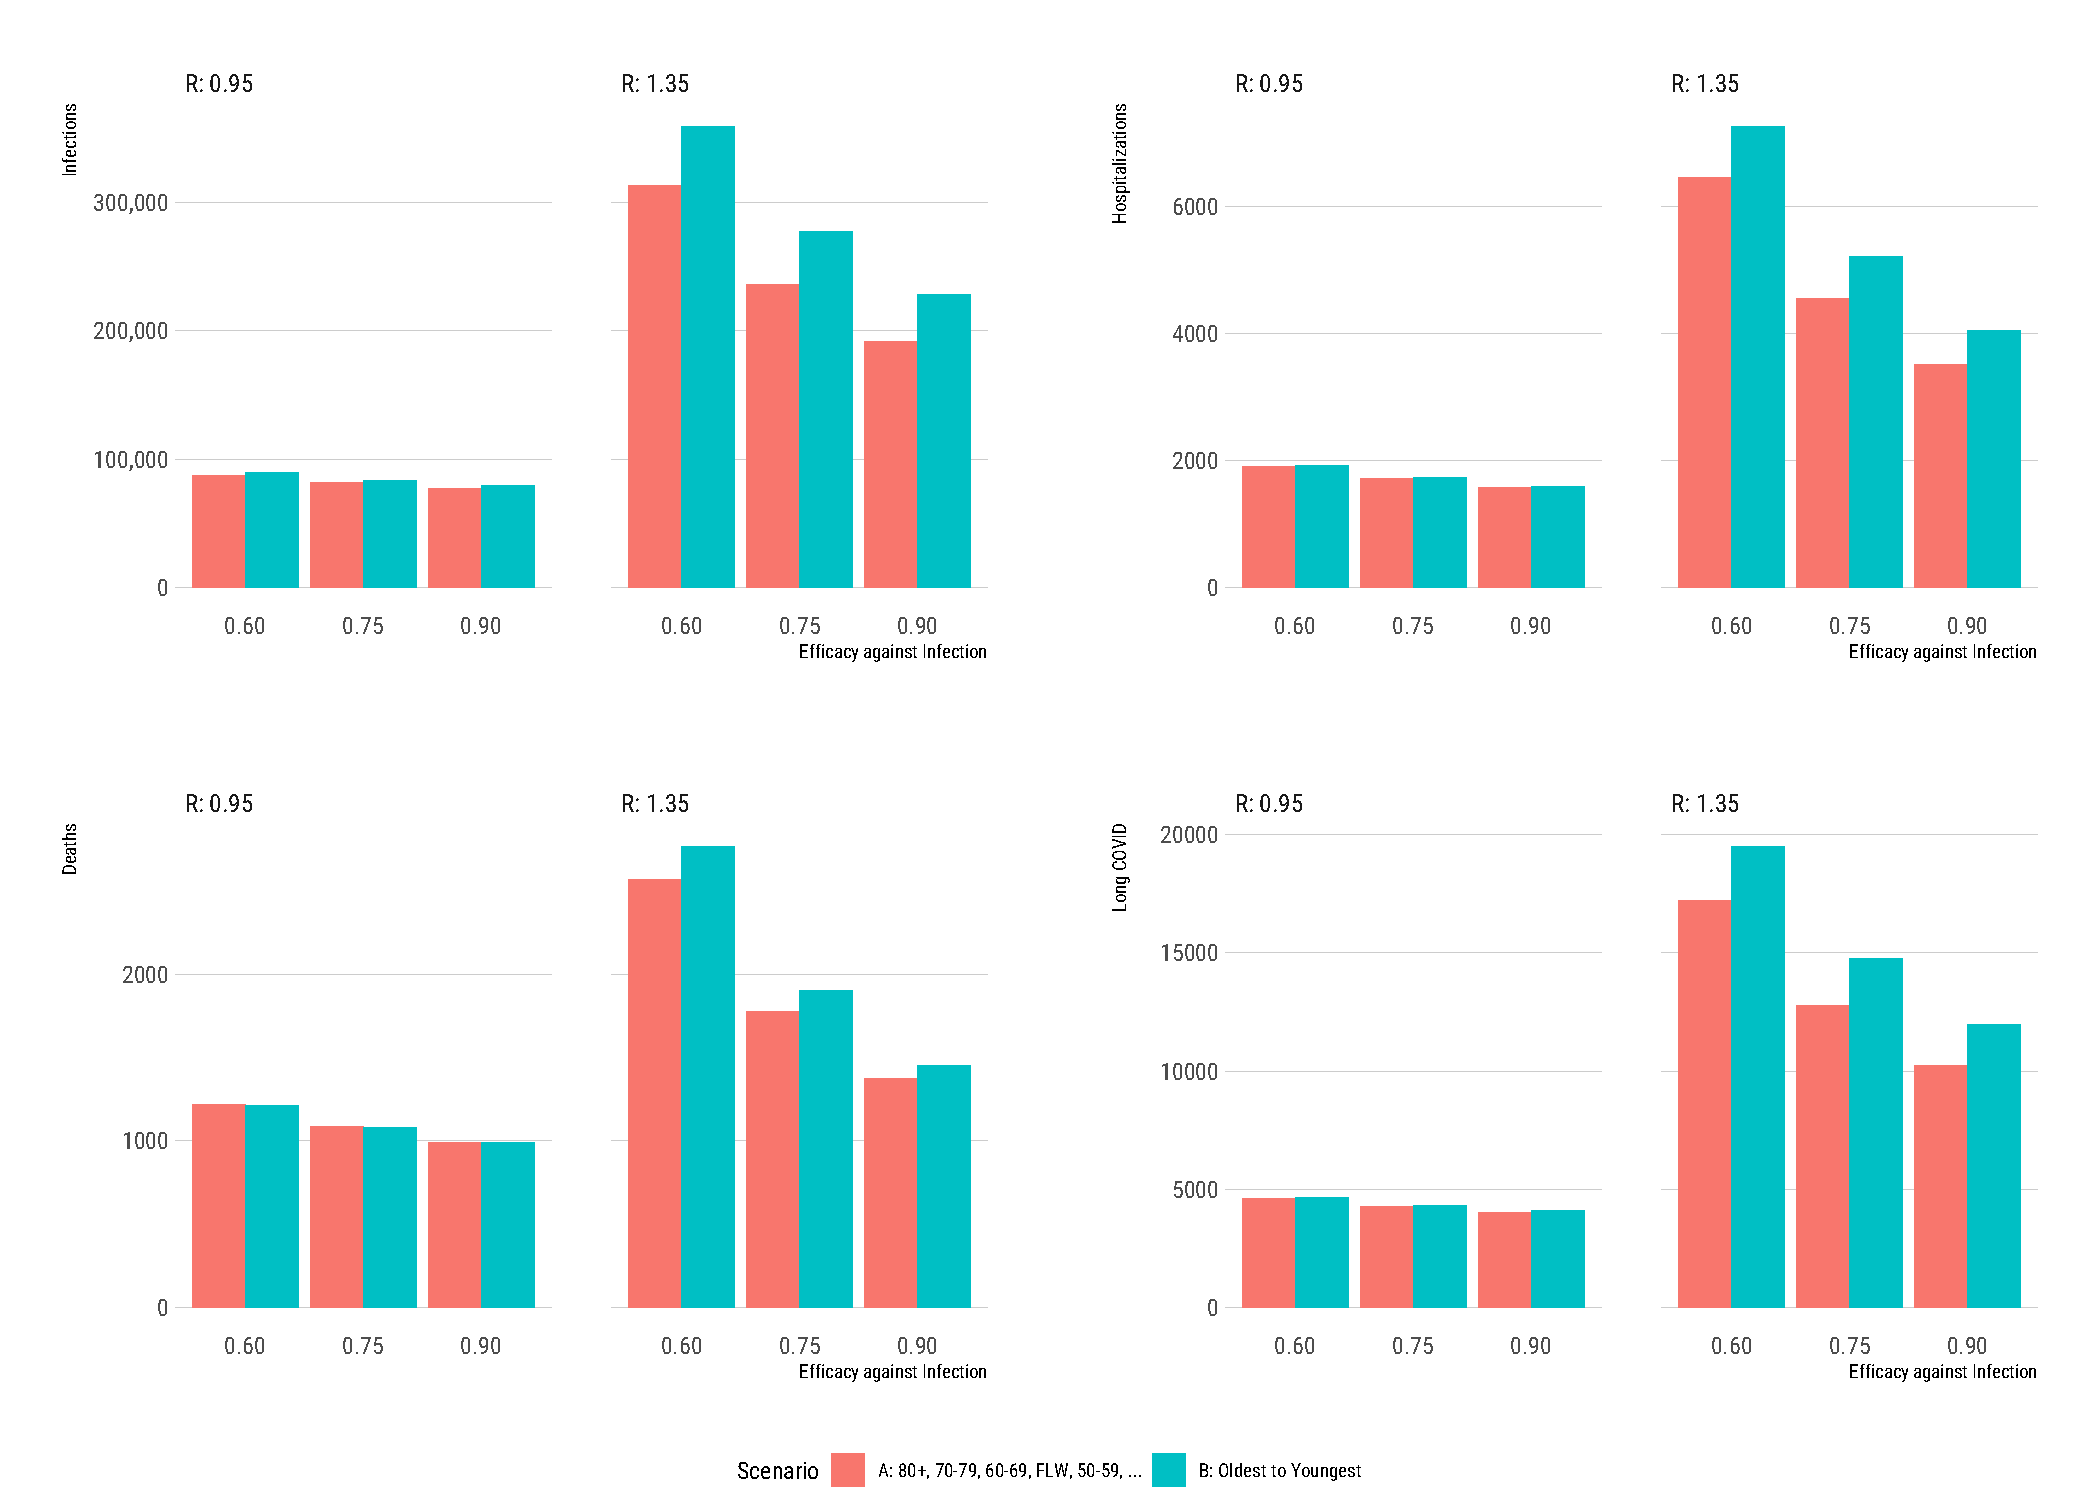
\includegraphics[width=1\linewidth]{../figures/fig-barplots} 

}

\caption{COVID-19 outcomes under different vaccination scenarios}\label{fig:fig2}
\end{figure}

\hypertarget{harm-benefit-from-a-personal-perspective}{%
\subsection{Harm-Benefit From a Personal
Perspective}\label{harm-benefit-from-a-personal-perspective}}

Not all interventions that are net-beneficial at a societal level are
net-beneficial for each member of the society, as those who carry the
burden of the risk of adverse events may not be the same people who
benefit from mitigation of the risk from contracting COVID19.

In mathematical terms, we compared \[
\begin{aligned}
P(death)_{VIPIT}  &= P(AZ) \times P(VIPIT|AZ) \times P(death|VIPIT, AZ) \\
P(death)_{delayedVaccination} &= P(COVID-19) \times P(death|COVID-19)
\end{aligned}
\] where \(P(AZ)\) is the probability of getting the AstraZeneca vaccine
(assumed to be 1 here), and \(P(COVID-19)\) is the probability of
contracting COVID-19 due to delayed vaccination.

We used results from our compartmental model to project mortality risk
from COVID-19 due to delayed vaccination.

\begin{figure}

{\centering 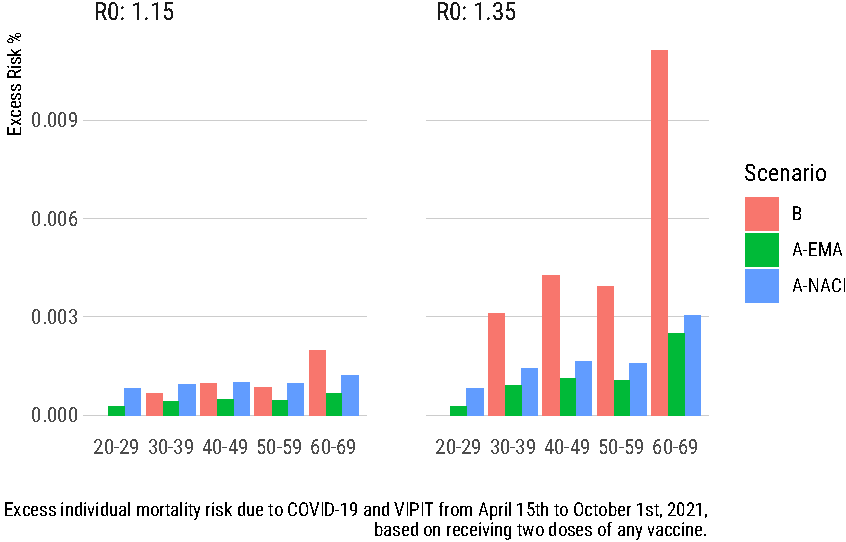
\includegraphics[width=0.7\linewidth]{theCaseforAZ_files/figure-latex/covidvsvipit-1} 

}

\caption{Mortality risk comparison for different age groups}\label{fig:covidvsvipit}
\end{figure}

Figure 3 compares the risk of VIPIT-related mortality from 2 doses of
the AstraZeneca vaccine with the mortality risk from COVID-19 due to
delayed vaccination. We did the comparison under two scenarios of
\(R_0\) of either 1.15 or 1.30, to represent different intensities for
the third wave, or alternatively to represent different geographical
parts of the province during the third wave. We found that under both
scenarios, the mortality risk due to COVID-19 to be much higher than the
highest estimate of the mortality associated with the risk for VIPIT in
40-49 and 50-59 age groups. Mortality risk from COVID-19 was also higher
for 30-39 age group, although the difference was negligible under
\(R_0\) of 1.15 scenario. For the 20-29 age group, the estimated risk of
vaccination with the AstraZeneca vaccine was higher than that of
COVID-19 from April 1st to July 1st, 2021.

\hypertarget{discussion}{%
\section{Discussion}\label{discussion}}

In its analysis of AstraZeneca vaccine, NACI weighed the risk of adverse
events against the age-stratified risk of mortality due to COVID-19,
pending an overall risk-assessment. However, the benefits of the
AstraZeneca vaccine go beyond preventing COVID-related mortality and
include protection against more common COVID complications in younger
adults including severe disease, hospitalizations, and Long COVID. The
recent sharp decline of COVID-19 cases in the UK suggests that the
AstraZeneca vaccine might also prevent onward transmission of the virus
\citep{our_world_in_data_covid-19_2021}.

The number of confirmed daily COVID-19 cases in the UK has plummeted
from about 60,000 cases a day in early January 2021 when a national
lockdown was imposed and about 3\% of the population had received at
least one vaccine dose, to about 11,000 cases per day on February 22,
2021 when a roadmap to easing lockdowns was announced to about 6000
cases per day on March 8, 2021 when the first phase of easing public
health restrictions was commenced \citep{bbc_lockdown_2021} and has
continuously declined since then to just above 4500 cases as of April 2,
2021 (47\% of the UK population have so far received one dose of a
COVID-19 vaccine). As about half of all vaccine doses administered in
the UK have been AZ vaccines, and based on the estimated AZ vaccine
efficacy of about 76\% against symptomatic COVID-19 and 64\% against any
NAAT-positive COVID-19 infection between 22 and 90 days after the first
dose \citep{voysey_single-dose_2021}, and real-world single-dose AZ
vaccine effectiveness of about 60\% against symptomatic COVID-19 and
80\% against COVID-19 hospitalization
\citep{public_health_england_1public_2021}, it is suggested that the AZ
vaccine is effective in reducing the overall burden of COVID-19.

Potential prevention of onward transmission with the AstraZeneca vaccine
could be especially critical for front-line workers during the current
wave of COVID cases. Of note, two recent studies from Toronto, Ontario
have shown that neighbourhoods with the highest proportion of essential
workers had per capita COVID-19 case and death rates that were 2.5-3
folds higher than that of neighborhoods with the lowest share of
essential workers
\citep[\citet{rao_disproportionate_2021}]{chagla_characterizing_2021}.

Based on our analysis from a societal perspective and assuming a
consequentialist framework, immediately making the AstraZeneca vaccine
available to essential workers is, assuming optimal uptake,
net-beneficial by a wide margin. Our analysis from a personal
perspective shows that the risk of contracting COVID-19 and dying from
it due to delayed vaccination is at least two times higher than the risk
of dying from VIPIT in those over 40, and also in those who are over 30
in large outbreak areas.

\hypertarget{doing-vs.-allowing-harm}{%
\subsection{Doing vs.~Allowing Harm}\label{doing-vs.-allowing-harm}}

For a public health intervention to be deemed ethically acceptable,
being net-beneficial at a societal level is not enough in and of itself.
As tragic as COVID-19 related mortality is, some hold that such events
are not comparable to causing death of otherwise healthy people because
of known even if rare side effect of a vaccine. as famously demonstrated
in the Trolley Problem, some people intuitively hold that causing harm
in worse than allowing harm, while others believe that at the end of the
day the consequences matter providing that the intention is benevolent.

The scope of this manuscript and our lack of expertise in this area
prevents us from doing justice to this important dilemma, and we refer
the interested reader to the appropriate literature
\citep{woollard_doing_2016}.

However, we believe that our conclusions hold regardless of the position
we take with respect to this ethical dilemma, as long as the expected
benefit outweighs the harm \emph{at a personal level}, as seems to be
the case for most age groups in our study.

Either way, all potential risks and latest evidence should be clearly
communicated with recipients before an informed consent is sought.

\hypertarget{communications-and-vaccine-hesitancy}{%
\subsection{Communications and Vaccine
Hesitancy}\label{communications-and-vaccine-hesitancy}}

Each time a recommendation for vaccine safety is reversed, there might
be a penalty in public trust, which could fuel vaccine hesitancy. Even
if a vaccination program is net beneficial from both a societal and a
personal perspective, vaccine side effects are likely to attract more
news coverage and attention on social media. Potential impacts of
COVID-19 vaccine roll-out on vaccine hesitancy, regardless of them being
positive or negative, might spill over into public perception of the
routine vaccination programs for the years to come.

\hypertarget{limitations}{%
\section{Limitations}\label{limitations}}

We did not consider ethical aspects of vaccine roll-out, and factors
such as uptake and vaccine hesitancy, as they were beyond our expertise.
Our analysis is based on currently available estimated rates of 1 in
million to 1 in 100,000 for VIPIT and might need correction should
higher rates of this complication be reported.

We have not considered potential sex differences in the risk for VIPIT.
Although cases identified to date have been predominantly female, it
remains unclear whether this was due to more females receiving the
AstraZeneca vaccine or due to an intrinsic difference in risk.

\hypertarget{conclusions}{%
\section{Conclusions}\label{conclusions}}

Immediate prioritization of front-line workers save lives. The optimum
strategy is, if logistically feasible, is to make Pfizer-BioNTech or
Moderna vaccine immediately available to essential workers and
reallocate the AstraZeneca vaccine for older individuals. If that is not
possible, continuing vaccination of front-line workers using AstraZeneca
vaccine is net-beneficial at a societal level. At a personal level,
current evidence suggests mortality risk posed by VIPIT is significantly
lower that mortality risk of contracting COVID-19 due to delayed
vaccination for 40-59 years old adults and for 30-39 adults who live in
an areas with larger outbreaks.

Ultimately, in dynamic situations like this where the evidence is
uncertain and evolving, vaccine roll-out decision are judgment calls
that need to take a complex network of medical, epidemiological,
ethical, logistics, and societal considerations into account.

\bibliographystyle{tfcad}
\bibliography{AZVIPIT.bib}




\end{document}
